\documentclass[12pt,a4paper]{ctexart}
\usepackage[utf8]{inputenc}
\usepackage{amsmath}
\usepackage{amsfonts}
\usepackage{amssymb}
\usepackage{graphicx}
\usepackage{hyperref}
\usepackage{listings}
\usepackage[left=2.00cm, right=2.00cm, top=2.00cm, bottom=2.00cm]{geometry}
\author{张吉祥}
\begin{document}
\paragraph{习题1}
\begin{enumerate}
	\item 当 $ rank(A) = rank(b) $ 时有唯一解;当 $ rank(A) > rank(b) $ 时有多解;当 $ rank(A) < rank(b) $ 时无解。
	\item 高斯分布:$ f(x)=(\sqrt{2\pi}\sigma)^{-1}\exp^{-\frac{(x-\mu)^{2}}{2\sigma^{2}}} $; $ f_{\mathbf{X}}(x_{1},\cdots,x_{k})=\dfrac{exp(-\frac{1}{2}(\mathbf{x}-\mathbf{\mu})^{T}\Sigma^{-1}(\mathbf{x}-\mathbf{\mu}))}{\sqrt{|2\pi\Sigma}|} $
	\item 初步了解C++的类和\textbf{STL},但还未用过
	\item 以前用过的编辑器有VC6.0、Xcode、Sublime Text和Vim
	\item 从\cite{Lippman2012}了解到C++11标准,新特性包括:\textbf{正则表达式、智能指针等},新标准还有C++14, C++17
	\item 熟悉Linux(Ubuntu),本科期间用过Ubuntu来学习和调试基于ROS的移动机器人
	\item 查看Linux目录结构 \textbf{\$ls /}。常用命令:\textbf{ls, cat, pwd, cd, make, mv, tar...}
	\item Ubuntu中常用apt安装软件,macOS常用brew安装软件。前者默认安装路径:PATH=/home/brightman/bin:/usr/local/sbin:/usr/local/bin:/usr/sbin:/usr/bin:/sbin:/bin:/usr/games;后者 Homebrew 会将软件包安装到独立目录,并将其文件软链接至 /usr/local。以安装\textbf{Eigen}库为例,源码安装 \footnote{Eigen只有头文件故不用编译} 或 \textbf{brew install eigen}
	\item \textbf{Vim}\footnote{不要在它的插件上浪费时间,不要想着把VIM用成IDE,我们只用它做文本编辑的工作} \textbf{\$ vimtutor}。执行外部命令\textbf{:!command}
	\begin{quote}
		\texttt{切记在使用中学习,而不是在记忆中学习}
	\end{quote}
\end{enumerate}

\paragraph{习题2}
\begin{enumerate}
	\item \cite{LiuHaoMin2016,梁明杰2013基于图优化的同时定位与地图创建综述}
	\item \cite{Cadena2016},\cite{Chen2007a},\cite{Chen2012b},\cite{Boal2014},\cite{Fuentes-Pacheco2015}。这些文献关于SLAM的看法与\cite{Gao2017SLAM}的异同:
	\begin{itemize}
		\item ...ToDo
		\item ...ToDo
	\end{itemize}
	\item \textbf{g++}命令参数举例:
	\begin{verbatim}
	$ g++ -o main main.cpp -I /头文件路径 -L /库文件路径 -l 库文件名称
	\end{verbatim}
	\item \textbf{Qt Creator}配置build文件夹
	\begin{verbatim}
	./%{JS: Util.asciify("build")}
	\end{verbatim}
	\begin{figure}
		\centering
%		\includegraphics[width=0.7\linewidth]{Img/debug}
		\caption{两个可执行程序时,在\textbf{Debug}前提下选helloSLAM或useHello}
		\label{fig:debug}
	\end{figure}
	\item 语法错误的情况下,\textbf{cmake}不能检测出来\footnote{cmake的功能是根据库的依赖关系生成\textbf{Makefile}文件,却不检查依赖关系是否完善?},\textbf{make}才会提示语法错误。
	\item \textbf{cmake}通过,但是\textbf{make}是报错:
	\begin{verbatim}
	Undefined symbols for architecture x86_64:
	"printHello()", referenced from:
	_main in useHello.cpp.o
	ld: symbol(s) not found for architecture x86_64
	\end{verbatim}
	\item DONE
	\item \textbf{find\_package}\\
	把头文件和库文件安装在自定义路径时,\textbf{动态库\footnote{小技巧:用\textbf{otool -L main}代替\textbf{ldd main}}链接出错}提示:\footnote{解决方案,考虑链接到\textbf{静态库} TARGET\_LINK\_LIBRARIES(main /Users/zhangjixiang/slambook/lib/libmyhello.a) }\footnote{g++ -o main main.cpp -I /Users/zhangjixiang/slambook/include/myhello -L /Users/zhangjixiang/slambook/lib -l myhello}
	\begin{verbatim}
	dyld: Library not loaded: libmyhello.6.dylib
	Referenced from: /Users/zhangjixiang/Documents/Programs/myhello/build/./main
	Reason: image not found
	\end{verbatim}
	{ @rpath}\\
	Q:\textbf{一定要安装在/usr/local路径吗???}\\
	\begin{verbatim}
	"otool -D <file>" to view the install name of a dylib
	"otool -L <file>" to view the dependencies
	"otool -l <file> | grep LC_RPATH -A2" to view the RPATHs
	"install_name_tool -id ..." to change an install name
	"install_name_tool -change ..." to change the dependencies
	"install_name_tool -rpath ... -add_rpath ... -delete_rpath ..." to change RPATHs
	\end{verbatim}
	\footnote{install\_name\_tool -change libmyhello.6.dylib /Users/zhangjixiang/slambook/lib/libmyhello.6.dylib ./a.out}
	
	{ C和C++相互调用出错时的解决方案:}
	\textbf{Linking C and CXX files in CMake}
	\begin{verbatim}
	#ifndef F_H
	#define F_H
	
	#ifdef __cplusplus
	extern "C" {
	#endif
	
	void f();
	
	#ifdef __cplusplus
	}
	#endif
	
	#endif
	\end{verbatim}
	
	{ \texttt{The standard locations for dynamic libraries are ~/lib, /usr/local/lib, and /usr/lib.}}
	
	{ \textbf{总结:macOS locates dependent libraries using FULLPATH to each dylib.}
		解决方法有三种:}
	\begin{enumerate}
		\item \textbf{安装到系统目录/usr/local}
		\item 修改共享库的 FULLPATH \textbf{install name}
		\begin{verbatim}
		install_name_tool -id "new_install_name" libdummy.dylib
		\end{verbatim}
		\item 修改生成共享库的CMakeLists.txt
		\begin{verbatim}
		IF(APPLE)
		SET(CMAKE_INSTALL_NAME_DIR /Users/zhangjixiang/slambook/lib)
		SET(CMAKE_BUILD_WITH_INSTALL_RPATH ON)
		ENDIF(APPLE)
		\end{verbatim}
	\end{enumerate}
	参考资料:
	\begin{itemize}
		\item \href{http://log.zyxar.com/blog/2012/03/10/install-name-on-os-x/}{\color{red}Install name on OS X}
		\item \href{https://cmake.org/pipermail/cmake/2011-April/043826.html}{How do folks work with rpath on OS X using cmake?}
	\end{itemize}
	\textbf{FindHELLO.cmake}:Search the paths specified by the \textbf{HINTS} option
	\begin{verbatim}
	find_path(HELLO_INCLUDE_DIR libHelloSLAM.h /Users/zhangjixiang/slambook/include/myhello)
	find_library(HELLO_LIBRARY NAMES myhello HINTS /Users/zhangjixiang/slambook/lib)
	
	#set(HELLO_LIBRARY /Users/zhangjixiang/slambook/lib/libmyhello.dylib)
	
	if(HELLO_INCLUDE_DIR AND HELLO_LIBRARY)
	set(HELLO_FOUND TRUE)
	endif(HELLO_INCLUDE_DIR AND HELLO_LIBRARY)
	
	if(HELLO_FOUND)
	if(NOT HELLO_FIND_QUIETRY)
	message(STATUS "Found hello: ${HELLO_LIBRARY}")
	endif(NOT HELLO_FIND_QUIETRY)
	else(HELLO_FOUND)
	if(HELLO_FIND_REQUIRED)
	message(FATAL_ERROR "Could not find myhello library")
	endif(HELLO_FIND_REQUIRED)
	endif(HELLO_FOUND)
	\end{verbatim}
	
	参考:\href{https://stackoverflow.com/questions/12075371/cmake-find-library-custom-library-location}{\color{red}{\Large cmake - find\_library - custom library location}}\\
	\href{https://cmake.org/cmake/help/v3.0/command/find\_library.html}{find\_library}
	\item DONE
	\item 熟悉灵活使用自己的工具\textbf{Qt Creator},了解其它特性
	\item \textbf{Qt Creator}的\textbf{vim}编辑功能
\end{enumerate}

\paragraph{习题3}
\begin{enumerate}
	\item 
	\begin{equation}\label{key}
	RR^{T}=
	\begin{bmatrix}
	e_{1}^{T}e_{1}^{\prime} & e_{1}^{T}e_{2}^{\prime} & e_{1}^{T}e_{3}^{\prime}\\
	e_{2}^{T}e_{1}^{\prime} & e_{2}^{T}e_{2}^{\prime} & e_{2}^{T}e_{3}^{\prime}\\
	e_{3}^{T}e_{1}^{\prime} & e_{3}^{T}e_{2}^{\prime} & e_{3}^{T}e_{3}^{\prime}\\
	\end{bmatrix}
	\begin{bmatrix}
	e_{1}^{T}e_{1}^{\prime} & e_{2}^{T}e_{1}^{\prime} & e_{3}^{T}e_{1}^{\prime}\\
	e_{1}^{T}e_{2}^{\prime} & e_{2}^{T}e_{2}^{\prime} & e_{3}^{T}e_{2}^{\prime}\\
	e_{1}^{T}e_{3}^{\prime} & e_{2}^{T}e_{3}^{\prime} & e_{3}^{T}e_{3}^{\prime}\\
	\end{bmatrix}
	=
	\textbf{I}
	\end{equation}
	从投影\footnote{内积}的角度理解旋转矩阵,并利用单位和正交条件\footnote{一共有6个约束方程}
	
	\item \href{https://en.wikipedia.org/wiki/Rodrigues%27_rotation_formula}{Rodrigues' rotation formula}\\
		\begin{equation}\label{key}
		R(a,\theta)=I_{3 \times 3}\cos \theta +aa^{T}(1-\cos \theta)+a^{\wedge} \sin \theta
		\end{equation}
		\begin{figure}
			\centering
%			\includegraphics[width=0.7\linewidth]{Img/Rodrigues}
			\caption{}
			\label{fig:rodrigues}
		\end{figure}
		\item 
		\begin{equation}\label{key}
		p^{\prime} = [\cos \dfrac{\theta}{2},\textbf{n}\sin \dfrac{\theta}{2}][0, \textbf{v}][\cos \dfrac{\theta}{2},\textbf{n}\sin \dfrac{\theta}{2}]^{-1}
		\end{equation}
		其中$ s = [-\textbf{n}^{T}\textbf{v}\sin \dfrac{\theta}{2}\cos \dfrac{\theta}{2}+\textbf{v}^{T}\textbf{n}\sin \dfrac{\theta}{2}\cos \dfrac{\theta}{2}+(\textbf{n}\times \textbf{v})^{T}\textbf{n}\sin^{2} \dfrac{\theta}{2}, ...] = [0, ...]$
		\item 见图表
		\item 
\lstset{language=C++}
\begin{lstlisting}
#include <iostream>
using namespace std;

#include <Eigen/Core>
#define MATRIX_SIZE 4

int main(int argc, char** argv)
{
	Eigen::Matrix<double, MATRIX_SIZE, MATRIX_SIZE> matrix_NN;
	matrix_NN = Eigen::MatrixXd::Random(MATRIX_SIZE, MATRIX_SIZE);
	cout << "Original Matrix = \n" << matrix_NN << endl;
	
	Eigen::Matrix3d matrix_I = Eigen::Matrix3d::Identity();
	cout << "TopLeft33 of the Matrix = \n" << matrix_NN.topLeftCorner(3,3) << endl;
	
	matrix_NN.topLeftCorner(3, 3) = matrix_I;
	cout << "Final Matrix = \n" << matrix_NN << endl;
	
	return 0;
}
\end{lstlisting}
		\item $ \textbf{Ax=b} $ 求解方法:
		\begin{itemize}
			\item Direct Methods
			\item Iteration Methods
		\end{itemize}
		\item 程序\footnote{\textbf{pretranslate()}:Applies on the \textbf{left} the translation matrix represented by the vector other to *this and returns a reference to *this. \textbf{translate()}:Applies on the \textbf{right} the translation matrix represented by the vector other to *this and returns a reference to *this.}:
		\lstset{language=C++}
\begin{lstlisting}
#include <iostream>
using namespace std;

#include <Eigen/Core>
#include <Eigen/Geometry>

#define MATRIX_SIZE 4

int main(int argc, char** argv)
{
	Eigen::Vector3d p_c1(0.5,0,0.2);
	Eigen::Vector3d p_c2;
	
	Eigen::Quaterniond q1(0.35, 0.2, 0.3, 0.1);
	q1.normalize();
	Eigen::Vector3d t1(0.3,0.1,0.1);
	Eigen::Isometry3d T_c1w = Eigen::Isometry3d::Identity();
	T_c1w.rotate(q1);
	T_c1w.pretranslate(t1);
	
	
	Eigen::Quaterniond q2(-0.5, 0.4, -0.1, 0.2);
	q2.normalize();
	Eigen::Vector3d t2(-0.1,0.5,0.3);
	Eigen::Isometry3d T_c2w = Eigen::Isometry3d::Identity();
	T_c2w.rotate(q2);
	T_c2w.pretranslate(t2);
	
	p_c2 = T_c2w * (T_c1w.inverse()) * p_c1;
	
	// cout <<  q2.toRotationMatrix() << endl;
	// cout <<  T_c2w.matrix() << endl;
	cout << "p_c1 = \n" << p_c1 << endl;
	cout << "p_c2 = \n" << p_c2 << endl;
	
	return 0;
}
\end{lstlisting}	
\end{enumerate}


\paragraph{习题4}
\begin{enumerate}
	\item 群的四个条件:\textbf{封闭性、结合律、幺元、逆},封闭性、结合律、幺元容易验证,只需验证逆:
	\begin{equation}\label{key}
	Sim(3)=
	\left\lbrace 
	S=
	\begin{bmatrix}
	sR&t\\
	0 &1\\
	\end{bmatrix}
	\in
	\mathbb{R}^{4\times 4}
	\right\rbrace 
	\end{equation}
	则
	\begin{equation}\label{key}
	S^{-1}=
	\begin{bmatrix}
	\dfrac{R^{T}}{s}&-\dfrac{R^{T}}{s}t\\
	0 &1\\
	\end{bmatrix}
	\in Sim(3)
	\end{equation}
	\item 李代数的四个条件:\textbf{封闭性、双线性、自反性、雅可比等价}。
	证明:记\textbf{g}=($ R^{3},R,\times $)
	\begin{itemize}
		\item $ \forall a,b \in R^{3},a\times b\in R^{3} $, 故满足封闭性;
		\item $ \forall \textbf{a,b,c} \in R^{3}, m,n\in R $, 有:\\
		$ (m\textbf{a}+n\textbf{b})\times \textbf{c}=m(\textbf{a}\times \textbf{c})+n(\textbf{b}\times \textbf{c}),\quad \textbf{c}\times (m\textbf{a}+n\textbf{b})=m(\textbf{c}\times \textbf{a})+n(\textbf{c}\times \textbf{b}) $\\
		故满足双线性;
		\item $ \forall a\in R^{3}, a\times a=\textbf{0} $, 故满足自反性;
		\item $ \forall a,b,c\in R^{3} $, 有\\
		$ a\times(b\times c)+b\times(c\times a)+c\times(a\times b) = $\\
		$ b(a\cdot c)-c(a\cdot b) + c(b\cdot a)-a(b\cdot c) + a(c\cdot b)-b(c\cdot a)=\textbf{0}$, 故满足雅可比等价. 综上有\textbf{g}=($ R^{3},R,\times $)为李代数。
	\end{itemize}
	
	\item $ \mathfrak{so(3)} $和$ \mathfrak{se(3)} $满足李代数的四个条件:\textbf{封闭性、双线性、自反性、雅可比等价}? TODO
	\item TODO
		\begin{itemize}
			\item $$a^{\wedge}a^{\wedge}=...=aa^T-I$$
			\item $$a^{\wedge}a^{\wedge}a^{\wedge}=...=-a^{\wedge}$$
		\end{itemize}
	\item 因为
	$$
	\forall v\in R^{3}, \quad (Ra)^{\wedge}v=(Ra)\times v=(Ra)\times(RR^{-1}v)=R[a\times (R^{-1}v)]=Ra^{\wedge}R^{-1}v
	$$, 且$ R^{-1}=R^{T} $, 故成立。$ \blacksquare $
	
	\item 记$ p=\theta a $, 原式左边:
	$$
	=R[\cos \theta \textbf{I}+(1-\cos \theta)aa^{T}+\sin\theta a^{\wedge}]R^{T}=\cos\theta\textbf{I}+(1-\cos\theta)R(aa^{T})R^{T}+\sin\theta(Ra^{\wedge}R^{T})
	$$
	$$
	=\cos\theta\textbf{I}+(1-\cos\theta)R(aa^{T})R^{T}+\sin\theta(Ra)^{\wedge}
	$$
	原式右边:
	$$
	=\cos \theta \textbf{I}+(1-\cos \theta)(Ra)(Ra)^{T}+\sin\theta (Ra)^{\wedge}
	=\cos\theta\textbf{I}+(1-\cos\theta)R(aa^{T})R^{T}+\sin\theta(Ra)^{\wedge}
	$$. 故等式左边$ = $右边, 即:
	\begin{equation}
	R\exp(p^{\wedge})R^{T}=\exp((Rp)^{\wedge})
	\end{equation}
	故原式成立。$ \blacksquare $
	
	\textbf{SE(3) 伴随性质证明}:\\
	原式左边:
	$$
	=
	\begin{bmatrix}
	R & t \\
	0 & 1 \\
	\end{bmatrix}
	\begin{bmatrix}
	\sum_{1} & \sum_{2} \\
	0 & 1 \\
	\end{bmatrix}
	\begin{bmatrix}
	R^{T} & -R^{T}t \\
	0 & 1 \\
	\end{bmatrix}
	=
	\begin{bmatrix}
	R\sum_{1}R^{T} & R\sum_{1}(-R^{T}t)+R\sum_{2}+t \\
	0 & 1 \\
	\end{bmatrix}
	$$, 式中$ \sum_{1}=\sum_{n=0}^{\infty}\frac{1}{n!}(\phi^{\wedge})^{n},\quad \sum_{2}=\sum_{n=0}^{\infty}\frac{1}{(n+1)!}(\phi^{\wedge})^{n}\rho $
	
	原式右边:
	$$
	=\exp(
	\begin{bmatrix}
	R\rho+(t^{\wedge}R)\phi \\
	R\phi \\
	\end{bmatrix}^{\wedge})
	=
	\begin{bmatrix}
	\sum_{3} & \sum_{4} \\
	0        & 1    \\
	\end{bmatrix}
	$$, 式中$ \sum_{3}=\sum_{n=0}^{\infty}\frac{1}{n!}((R\phi)^{\wedge})^{n},\quad \sum_{4}=\sum_{n=0}^{\infty}\frac{1}{(n+1)!}((R\phi)^{\wedge})^{n}[R\rho+t^{\wedge}R\phi] $. \\
	故只需要证明:
	$$
	\sum_{3}=R\sum_{1}R^{T}, \quad \sum_{4}=R\sum_{1}(-R^{T}t)+R\sum_{2}+t
	$$, 其中$ \sum_{3}=R\sum_{1}R^{T} $显然成立。下面证明$ \sum_{4}=R\sum_{1}(-R^{T}t)+R\sum_{2}+t $:\\
	原式等价于
	$$
	\Leftrightarrow
	\sum_{n=0}^{\infty}\frac{1}{(n+1)!}((R\phi)^{\wedge})^{n}[R\rho+t^{\wedge}R\phi] = -\sum_{n=0}^{\infty}\frac{1}{n!}((R\phi)^{\wedge})^{n}t+R\sum_{n=0}^{\infty}\frac{1}{(n+1)!}(\phi^{\wedge})^{n}\rho+t
	$$
	$$
	\Leftrightarrow
	\sum_{n=0}^{\infty}\frac{1}{(n+1)!}((R\phi)^{\wedge})^{n}[t^{\wedge}R\phi] =
	-\sum_{n=0}^{\infty}\frac{1}{n!}((R\phi)^{\wedge})^{n}t+t
	$$
	$$
	\Leftrightarrow
	\sum_{n=0}^{\infty}\frac{1}{(n+1)!}((R\phi)^{\wedge})^{n}[-(R\phi)^{\wedge}t] =
	-\sum_{n=0}^{\infty}\frac{1}{n!}((R\phi)^{\wedge})^{n}t+t
	$$
	$$
	\Leftrightarrow
	-\sum_{n=0}^{\infty}\frac{1}{(n+1)!}((R\phi)^{\wedge})^{n+1}t =
	-\sum_{n=0}^{\infty}\frac{1}{n!}((R\phi)^{\wedge})^{n}t+t
	$$, 故等式成立。$ \blacksquare $
	
	\item 
		\begin{itemize}
			\item \textbf{SO(3)右扰动模型}(图\ref{fig:so3})
			\begin{figure}[tbph!]
				\centering
				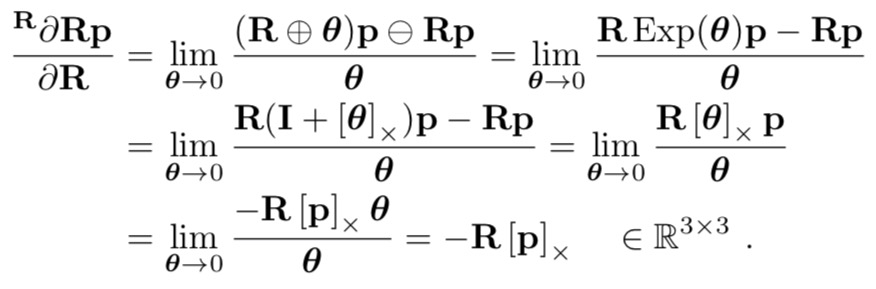
\includegraphics[width=0.7\linewidth]{so3}
				\caption{SO(3)右扰动模型}
				\label{fig:so3}
			\end{figure}
			\item \textbf{SE(3)右扰动模型} TODO
		\end{itemize}
	\item 
	\begin{verbatim}
	find_package(<package> [version] [EXACT] [QUIET] [MODULE]
	[REQUIRED] [[COMPONENTS] [components...]]
	[OPTIONAL_COMPONENTS components...]
	[NO_POLICY_SCOPE])
	\end{verbatim}
	
	Command \textbf{find\_package} has two modes: \textbf{Module mode} and \textbf{Config mode}.
\end{enumerate}

\end{document}